\chapter{Machine Learning Pipelines}
Recall the pipeline diagram from the first chapter.

\begin{figure}[h]
  \centering
  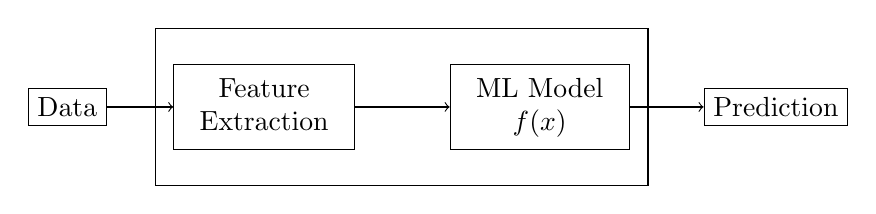
\begin{tikzpicture}
    \node[draw, rectangle] (data) at (0, 0) {Data};
    \node[draw, rectangle] (features) at (2.5, 0) {\begin{tabular}{c}Feature\\Extraction\end{tabular}};
    \node[draw, rectangle, minimum height=2cm, minimum width=6.25cm] () at (4.25, 0) {};
    \node[draw, rectangle] (model) at (6, 0) {\begin{tabular}{c}ML Model\\$f(x)$\end{tabular}};
    \node[draw, rectangle] (prediction) at (9, 0) {Prediction};
    \draw[->] (data) -- (features);
    \draw[->] (features) -- (model);
    \draw[->] (model) -- (prediction);
  \end{tikzpicture}
  \caption{Machine Learning Pipeline}
  \label{fig:ml-pipeline}
\end{figure}
Up until now we always assumed to have a vector representation $\vec{x}\in\mathbb{R}^d$ of our data.
Starting from now, our data might be in any other format, like text or images.

To build a system that gets a certain format of input, transform this input into $d$ dimensional vectors and feeds them into our model.
We will now look at how to program such an ML-Pipeline
\section{Motivation}
In the previous chapters we looked into different feature extraction techniques.
We also looked in previous chapters into different ML models and how to train them.
Now, we will look into how to combine these two concepts into a single pipeline.

One way how to implement this is to manually write code that executes all steps of the pipeline sequentially.
But this would be quite static and not very flexible. We would need to rewrite the code for every new data set or whenever
we want to change a part of the pipeline.

A better way to implement this is to use a so called \textit{Pipeline} object. This object is a wrapper around all steps of the pipeline.
The most popular API-Interface~\cite{sklearn_api} for this is implemented by the guys from scikit-learn~\cite{scikit-learn}.

We will look into the implementation of such a pipeline in the following because it will allow to combine
own implementations with implementations inside scikit-learn. This is especially useful because scikit-learn
delivers plenty of tools, feature extraction algorithms and model architectures.

I personally work a lot with scikit-learn and I highly recommend it to anyone who wants to get started with ML as well assigned
encourage everyone to contribute to the project.

\section{Estimators}
\framedtext{\color{red}{TODO:}}

